\section{Experiments}

This section reports on \system experiments in an Ubuntu 16.04.4 LTS OS running in $04$ cores of local $i7~3.7$GHz processors with 08 Gb RAM.
Particularly, we evaluated \system in a set of experiments on \dataset for 
\textit{(i)}~tuning \system first phase,
\textit{(ii)}~addressing the gains of pixelwise classification,
\textit{(iii)}~tuning \system second phase, and
\textit{(iv)}~assessing \system quality in tissue segmentation.\\

\noindent
\textbf{Tuning of \system first phase.}
We experimented on $40$ labeled \dataset images for the tuning of \system classification phase.
Image pixels were manually separated into background and skin pixels resulting in more than 100 million points, which were sampled, with stratification by class, into sets of $1 \cdot 10^1, 1 \cdot 10^2, 1 \cdot 10^3, 1 \cdot 10^4$ and $1 \cdot 10^5$ pixels.
Figure~\ref{fig:sample} shows the RGB plots for samples $1 \cdot 10^3, 1 \cdot 10^4$ and $1 \cdot 10^5$, in which points are divided into two separated groups.

\begin{figure}[!htb]
\centering
\includegraphics[scale=1.02]{figs/plots.pdf}
\caption{RGB points for samples
(a)~$1 \cdot 10^3$,
(b)~$1 \cdot 10^4$, and
(c)~$1 \cdot 10^5$.}
\label{fig:sample}
\end{figure}

\begin{figure*}[!htb]
\centering
\includegraphics[scale=.84]{figs/res2.pdf}
\vspace{-6px}
\caption{Bar plots for \system second phase tuning, and two wound segmentation examples for increasing $L_1$-based DBSCAN similarity thresholds.}
\label{fig:expto_dbscan}
\end{figure*}

Such a two-class pixel classification problem was addressed through 10-folds cross-validation tests over classifiers previously used in related works, namely Na\"{i}ve-Bayes (NB), Bayes-Net (BN), Instance-based Learning (IbL), Multi-Layer Perceptron with Levenberg--Marquardt (MLP-LM) and Rprop training algorithms (LMP-RP), Decision-Tree (DT), and RandomForest (RF).
Table~\ref{tab:classifiers} shows the scores of Cohen-Kappa Coefficient (CKC) for each classifier and indicates MLP-LM and RF outperformed the competitors in most of the samples (bold column values).
Accordingly, we selected MLP-LM as the \system first phase classifier as it reached the best scores for both weighted ($\bar{\mu}$) and simple ($\mu$) CKC mean.
Although only CKC is reported due to space limitations, MLP-LM also reached the highest ratings for weighted classification metrics Sensitivity ($.98$) and Specificity ($.98$).
\vspace{-10px}

\begin{table}[!htb]
\centering
\caption{Cohen-Kappa Coefficient (CKC) for \system first phase.}
\vspace{-5px}
\label{tab:classifiers}
\begin{tabular}{l|c|c|c|c|c||c|c} \hline \hline
 & 
\multicolumn{7}{c}{ {\cellcolor[HTML]{68CBD0}\textbf{Sample Size}} }    \\ \hline
\cellcolor[HTML]{68CBD0} \textbf{Classifier} & 
\cellcolor[HTML]{68CBD0} \textbf{$10^1$}  & 
\cellcolor[HTML]{68CBD0} \textbf{$10^2$}  & 
\cellcolor[HTML]{68CBD0} \textbf{$10^3$}  & 
\cellcolor[HTML]{68CBD0} \textbf{$10^4$}  & 
\cellcolor[HTML]{68CBD0} \textbf{$10^5$}  &
\cellcolor[HTML]{68CBD0} \textbf{$\bar{\mu}$} &
\cellcolor[HTML]{68CBD0} \textbf{$\mu$}\\ \hline \hline
NB         & .156 & .710 & .793 & .797 & .805  & .804 & .652 \\ \hline
BN         & .038 & .423 & .639 & .722 & .743  & .739 & .513 \\ \hline
%DS         & .025 & .541 & .443 & .408 & .411  & .411 & .365 \\ \hline
IbL        & .675 & .874 & \textbf{.967} & \textbf{.967} & .971 & .970 & .890\\ \hline
\textbf{MLP-LM} & \textbf{.697} & \textbf{.895} & .953 & \textbf{.967} & \textbf{.972} & \textbf{.971} & \textbf{.896} \\ \hline
MLP-RP     & .423 & .829 & .929 & .958 & .968  & .967 & .821 \\ \hline
DT         & .493 & .790 & .922 & \textbf{.967} & .970  & .969 & .828 \\ \hline
%RT         & .217 & .855 & .941 & .964 & .970  & .969 & .789 \\ \hline
RF         & .350 & .854 & .947 & \textbf{.967} & \textbf{.972} & \textbf{.971} & .818\\ \hline \hline
\end{tabular}
\end{table}

\noindent
\textbf{Discarding of superpixels.}
We measured the impact of background removal by calculating the number of regions of interest eliminated from \system second phase after the pixelwise classification.
Figure~\ref{fig:efic} shows the mean and standard deviation for the proportion of discarded regions of interest in a varying number of superpixels ($K_p$) regarding $40$ images.
The higher the discard ratio, the more efficient is \system for eliminating candidate regions.
Consolidated results indicate discarding ratio grew linearly to the number of superpixels and reached up to $48\%$ of dismissed regions for $K_p = 10 \cdot 10^3$.\\

\noindent
\textbf{Tuning of \system second phase.}
We evaluated the impact of two DBSCAN parameters upon $40$ \dataset images with background removed by \system first phase.
In particular, we experimented on five metrics $\delta = L_1$, $L_2$, $L_\infty,$ Canberra, and BrayCurtis and $30$ thresholds ranging from $\xi = 0.5\%$ to $\xi = 15\%$ of maximum dissimilarity in steps of $0.5\%$.
Figure~\ref{fig:expto_dbscan} shows two segmentation examples for DBSCAN and the experimented settings.
Canberra and BrayCurtis presented a wider variance regarding the number of groups by thresholds, while functions $L_1$, $L_2$ and $L_\infty$ exhibited a stable behavior, \textit{i.e.}, lower variances. 
Function $L_1$ also generated fewer clusters in comparison to other metrics for all thresholds, on average.

\begin{figure}[!htb]
\centering
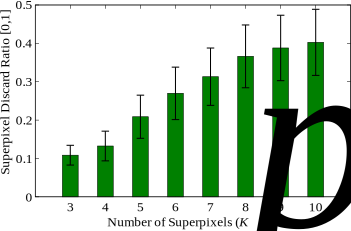
\includegraphics[scale=.68]{figs/efic.pdf}
\vspace{-8px}
\caption{\system first phase superpixel elimination ratio.}
\label{fig:efic}
\end{figure}

Figure~\ref{fig:expto_dbscan} also provides two examples of bar plots regarding the number of groups and the similarity thresholds.
Bar plots of evaluated images resembled an exponential decay function, whose slope is leveling off towards the curve ``elbow''.
Accordingly, we took advantage of such behavior for applying the elbow criterion of Scree-Plot factor analysis~\cite{Jolliffe2011} for the setting of the DBSCAN threshold.
The premise is the curve elbow indicates where the bar plot starts to smooth up so that the cut point can be determined by the first of two consecutive bars whose difference ratio does not exceed a fixed threshold $\Delta, \Delta \leq \frac{bar_i - bar_{i+1}}{bar_i}$.

Hence, we experimented with $\Delta$ ranging from $5\%$ to $20\%$ of the bar difference ratio in steps of $1\%$, and the most frequent cut point regarding the $40$ evaluated images was the similarity threshold $\xi = 3\%$.
Figure~\ref{fig:expto_dbscan} highlights two examples of superpixel clustering (green borders) carried out by DBSCAN with these suitable settings, \textit{i.e.}, distance $\delta = L_1$, and threshold $\xi = 3\%$.\\

\noindent
\textbf{Pixelwise area quantification.} 
In the last experiment, we separated 04 new and diversified \dataset images that were manually segmented by an expert.
Figures~\ref{fig:quantification}(a--b) show one of the selected images and the expert-provided segmentation, while Figures~\ref{fig:quantification}(c--d) illustrate the outputs of \system first and second phase, respectively.
\system segmented pixels were matched to expert segmentation with a Mean Absolute Error (MAE) ratio of $.05$  (variance of $.01$), which indicates a high separation ratio through the divide-and-conquer strategy.

\begin{figure}[!htb]
\centering
\includegraphics[scale=.96]{figs/quantification1.pdf}
\vspace{-8px}
\caption{(a)~Example of an \dataset image, and
(b)~manual tissue segmentation.
(c)~\system first phase output, and
(d)~\system outcome.}
\label{fig:quantification}
\end{figure}





